%===============================================================================
% Main Latex 
% Configuration of Document
%===============================================================================
\documentclass[10pt,oneside,pdftex]{article}
\usepackage{graphics}
\usepackage[pdftex]{graphicx}
\usepackage{amsmath, amstext, amsfonts, amssymb}
\usepackage{fancyvrb}
\usepackage{setspace}
\usepackage{longtable} 
\usepackage{supertabular}
\usepackage{tabularx} 
\usepackage{multirow}
\singlespacing
\usepackage{color}
\definecolor{bl}{rgb}{0.0,0.2,0.6} 
\usepackage{sectsty}
\usepackage{url}
\usepackage{listings}
\usepackage[left=2.54cm,bottom=2.00cm,top=2.00cm,right=2.54cm]{geometry}
\usepackage[compact]{titlesec} 
%\allsectionsfont{\color{bl}\scshape\selectfont}
\allsectionsfont{\color{bl}}
\newcommand{\dirfig}{./images}
\usepackage[linktoc=all]{hyperref}
\hypersetup{
    colorlinks,
    citecolor=blue,
    filecolor=blue,
    linkcolor=blue,
    urlcolor=blue
}



%===============================================================================
% Fonts in Document
%===============================================================================
%\usepackage{times}
%\usepackage{pslatex}
%\usepackage{newcent}
%\usepackage{palatcm}
%\usepackage{palatino}
\usepackage[T1]{fontenc}
\usepackage[scaled]{helvet}
\renewcommand*\familydefault{\sfdefault}
%\renewcommand*{\encodingdefault}{T1}
% For more options go to: http://www.tug.dk/FontCatalogue/
\usepackage[colorinlistoftodos]{todonotes}

%===============================================================================
% Define a new command that prints the title only
%===============================================================================
\makeatletter                                           % Begin definition
\def\printtitle{                                        % Define command: \printtitle
{\color{bl} \centering \huge \sc \textbf{\@title}\par}} % Typesetting
\makeatother % End definition

\title{2. Free Energy Perturbation (FEP)}


%===============================================================================
% Define a new command that prints the author(s) only
%===============================================================================
\makeatletter                                           % Begin definition
\def\printauthor{                                       % Define command: \printauthor
{\centering \small \@author}}                           % Typesetting
\makeatother                                            % End definition

\author{
\vspace{10pt}
Updated by: Mauricio Esguerra\\
July 6, 2015\\
\vspace{10pt}
\small{based on an original version by:}\\
\small{Martin Alml\"of, Martin And\'er, Sinisa Bjelic, Jens Carlsson, Hugo Guti\'errez de Ter\'an,} \\
\small{Martin Nervall, Stefan Trobro and Fredrik \"Osterberg}\\
\vspace{20pt}
}


%===============================================================================
% Custom headers and footers
%===============================================================================
\usepackage{fancyhdr}
\pagestyle{fancy} % Enabling the custom headers/footers
\usepackage{lastpage}
% Header (empty)
\lhead{}
\chead{}
\rhead{}

% Footer (you may change this to your own needs)
\lfoot{\footnotesize Q Tutorials - \texttt{FEP}}
\cfoot{}
\rfoot{\footnotesize page \thepage\ }%of \pageref{LastPage}} % "Page 1 of 2"
\renewcommand{\headrulewidth}{0.0pt}
\renewcommand{\footrulewidth}{0.4pt}


%===============================================================================
% Begin Document
%===============================================================================
\begin{document}
\printtitle
\printauthor

\tableofcontents
%\newpage
\vspace{10 mm}
\renewcommand{\thefigure}{\arabic{figure}}

\bibliographystyle{nar}
\section{Free Energy Perturbation (FEP)}
Free  energy  perturbation simulations  can  be  used for  theoretical
prediction of binding free energies  and along with it the elucidation
and/or   prediction  of   chemical  reaction   mechanisms.   In   this
step-by-step tutorial you will be able to compute the relative binding
free energy of  camphane and camphor to an enzyme  which catalyzes the
addition  of   molecular  oxygen   to  nonactivated   hydrocarbons  at
physiological temperature. This oxydizing  enzyme is called cytochrome
P450 cam \cite{schlichting2000}.

\subsection{Theoretical background} 
The Free Energy Perturbation method is just that, a method, it is not,
by any  means, a theory. The  method, in broad lines,  allows a travel
between  states given  a  forced  path.  This  makes  sense since,  by
definition,  the Free  Energy of  a  system is  a thermodynamic  state
function  and therefore  its value  must  be independent  of the  path
taken.   An approximation  is made  that  a partition  function for  a
perturbed system can be separated  from the full partition function of
the system as given by equation  3.  The original expressions given by
Zwanzing \cite{zwanzig1954}  to describe the  idea of the  Free Energy
Perturbation (FEP) method as applied to hot gases are given below:

\begin{gather}
exp(-\beta\bar{A}_{N})=Q_{N}=\frac{1}{N!}    \int_{v}  ...    \int_{v}
\times
exp(-\beta V_{N}) d_{\tau 1} ... d_{\tau N} \\
V_{N}=V_{N}^{(0)} + V_{N}^{(1)}\\
exp-\beta(\bar{A}_{N}-\bar{A}_{N}^{(0)})\equiv
exp(-\beta\bar{A}_{N}^{(1)})\\
\label{eq:zwanzig}
exp(-\beta\bar{A}_{N}^{(1)})=\langle      exp(-\beta      V_{N}^{(1)})
\rangle_{0}
\end{gather}

Where $\beta = 1/ \kappa T$,  $\kappa$ is Boltzmann's constant, $T$ is
the temperature  in Kelvin, $Q_{N}$ is the  configurational partition
function of the system, $\bar{A}$  is the configurational free energy,
and $V_{N}$ is the total potential energy of the system.

Notice that the  paper is called ``High Temperature  Equation of State
by  a  Perturbation  Method.  I.   Nonpolar  Gases''.  Why  the  title
specifically states the high temperature case is because it deals with
a gas where  particles are not interacting with each  other and so can
be considered to be having fully elastic collisions.\\

A more modern notation to  describe the perturbation method as applied
to   free   energies   is    given   by   Pohorille,   Jarzynski   and
Chipot\cite{pohorille2010} in the following expression:
\begin{gather}
exp(-\beta\Delta A)= \langle exp(-\beta\Delta U) \rangle
\end{gather}

\noindent  Eq.   \ref{eq:zwanzig}  is  derived  from   the  statistical
mechanics expression for the Helmholtz free energy, \textit{A}, and the
configurational partition function integral, \textit {Z}.

\begin{equation}
\label{eq:s.m.h.}
  A=-kT \cdot \ln(Z)
\end{equation}

\begin{equation}
\label{eq:conf}
  Z=\int e^{-V/(kT)} d \Gamma
\end{equation}

\noindent At constant pressure and volume the change in Helmholtz free
energy equals  that in Gibbs  free energy. The free  energy difference
between the  two different states A  and B, that are  represented with
potential  energies $V_A$  and $V_B$  respectively, can  be rearranged
into the eq.  \ref{eq:zwanzig} as follows:


\begin{eqnarray}
  \nonumber \Delta G_{A \rightarrow B}&=&-(kT \cdot \ln(Z_B)-kT \cdot \ln(Z_A))\\
  \nonumber &=& -kT \cdot \ln(Z_B/Z_A)\\
             &=& -kT \cdot \ln((\int e^{-V_B/(kT)} d \Gamma)/(\int e^{-V_A/(kT)} d \Gamma))\\
  \nonumber &=& -kT \cdot \ln((\int e^{-V_B/(kT)}e^{-V_A/(kT)}e^{V_A/(kT)} d \Gamma)/(\int e^{-V_A/(kT)} d \Gamma))\\
  \nonumber &=& -kT \cdot \ln<e^{-\Delta V_{A \rightarrow B}/(kT)}>_A
\end{eqnarray}

FEP  is  very  accurate   concerning  small  perturbations,  when  the
difference  between the  potential  $V_A$ and  $V_B$  is smaller  than
2 kT. The  free energy of  association of the  ligands to a  protein is
calculated with FEP as a relative difference between the ligands.  The
absolute binding  energy is defined  as a free energy  associated with
moving the ligand in  water to a solvated protein, paths  II and IV in
Figure \ref{fig:fep}. The  relative binding energies are  defined as a
difference  between two  simulations where  the ligand  A is  stepwise
transformed to ligand B in water  and in solvated protein, paths I and
III in Figure \ref{fig:fep}.


\begin{figure}
\centering
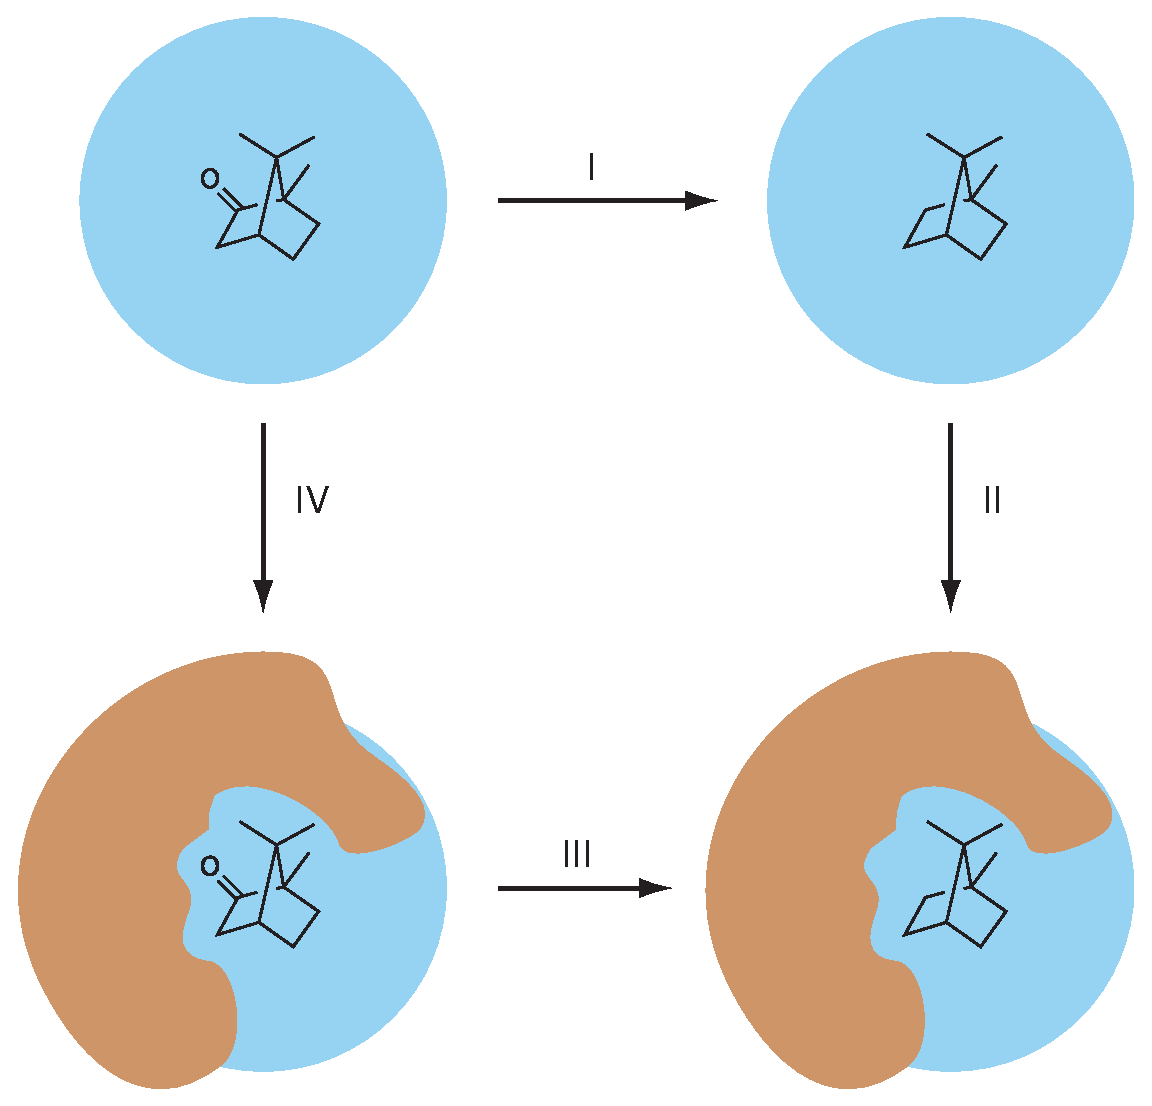
\includegraphics[width=7cm]{images/lie.eps}
\caption{\label{fig:fep}  Thermodynamic cycle  for  ligand binding  of
  camphene (CMA)  and camphor (CAM)  to the P450cam enzyme.  The brown
  blob denotes the enzyme, and the blue background represents water.}
\end{figure}
\newpage

\subsection{FEP simulations using \textbf{qdyn}}

Before starting the tutorial change the directory to \texttt{protein}
or \texttt{water} in the \texttt{FEP} folder.\\

In this tutorial  we are going to analyze the  perturbation of camphor
(CAM) to  camphane (CMA)  in water  and in  the P450cam  enzyme.  P450
enzymes catalyze the hydroxylation of unactivated alkanes, and P450cam
specifically  catalyzes the  hydroxylation of  camphor.  Although  the
system investigated  here is  P450cam the rules  in this  tutorial are
general and can be applied to any system of interest.

A FEP simulation  is specified in \textbf{Q}  with a \texttt{name.fep}
file   where  the   transformation  is   defined  in   detail.   Every
\texttt{name.fep} file is split into a number of sections where we can
define atoms, charges, bonds and  angles which are changing during the
FEP simulation (see Figure \ref{fig:fepfile}).  Note that a section in
\textbf{Q} follows the syntax $[$...$]$.\\

-  Open   the  \texttt{cma\_cam.fep} file,   in  the   \texttt{protein}  or
\texttt{water}   folder,   that  is   used   for   the  CMA   to   CAM
perturbation. Try  to locate the  different sections that are  used in
the FEP file. Can you understand how CMA is transformed to CAM?\\

- What effect do they have  on the simulation? (HINT: For the detailed
explanation of the different sections consult Appendix A!)\\


\begin{figure}[ht]
\texttt{
\\
$[$atoms$]$\\
...\\
\\
$[$FEP$]$\\
...\\
\\
$[$change\_charges$]$\\
...\\
\\
$[$atom\_types$]$\\
...\\
\\
.\\
.\\
.\\
}
\caption{\label{fig:fepfile}FEP file format.}
\end{figure}

Having a FEP file the perturbation is defined in Q by adding a
specifier
\\
\\
\texttt{ fep \hspace{2cm}    name.fep}
\\
\\
in the input files for \textbf{qdyn}. Additionally it is necessary to add
the section \texttt{$[$lambdas$]$} where the lambda values are
defined, $\lambda_1$ and $\lambda_2$. The lambda values are used
to transform the potential $V_A$ to $V_B$ in small steps to
improve the convergence. The energies are sampled on the potential
V,
\begin{equation}
\label{eq:lambda}
V=\lambda_1 V_A + \lambda_2 V_B = \lambda_1 V_A + (1-\lambda_1) V_B
\end{equation}
where $\lambda_1$ varies between 0 and 1. How many lambda steps
are used in the simulation depends on difference between
$V_A$ and $V_B$ and the type of perturbation.\\

- Open an input file \texttt{name.inp}. In what section is the fep file read?\\

- Find the \texttt{$[$lambdas$]$} section. How many lambda steps
are used in the perturbation and how big is each step? (HINT: Look
in several \texttt{cma\_camN.inp} files, where \texttt{N}=0..30.)\\

- How many steps are used in the simulation in each file?\\

- Also note the specifiers\\

\noindent \texttt{energy \hspace{2cm}             name.en}\\
\texttt{energy  \hspace{2cm}                 25}\\

\noindent that are used for saving the energies every 25th step to
the file \texttt{name.en}.
\newpage

\subsection{Analysis of FEP simulations using \textbf{qfep}}
All steps  in this  tutorial take approximately  2-3 hours  running in
parallel  in   eight  processor   cores  in   a  2.3   GHz  processor.
\textbf{qfep} is the analysis program  which allows you to compute the
free energy differences between states  using energies which have been
stored in the  binary files with ".en" extension, that  is, files such
as \texttt{cma\_cam30.en}.\\
To  run  qfep you  must  issue  the  following  command for  both  the
simulation in plain water and in the protein:

\begin{Verbatim}
qfep < qfep.inp > qfep.out
\end{Verbatim}

The \texttt{qfep.inp} file contains all necessary instructions issued
to \textbf{qfep} and the \texttt{qfep.out} contains the full output.\\

- Open \texttt{qfep.inp} and \texttt{qfep.out}. 
Try to understand the different commands.
What are they specifying? (HINT: Check out Appendix B!)\\

- The free energy difference for  the perturbation from CMA to CAM can
be found at  the end of table summarized in  \texttt{Part 1}.  What is
the difference between water and protein?\\

Water simulation: $\Delta G_{A \rightarrow B}^w=$ \hspace{2cm} (kcal/mol)\\

Protein simulation: $\Delta G_{A \rightarrow B}^p=$ \hspace{2cm}(kcal/mol)\\

The free  energy is calculated as  an average of forward  and backward
calculations  at every  lambda point.  The forward  and backward  free
energy  values  are also  summarized  in  \texttt{Part   1}  of  the
\texttt{qfep.out}    file    in    columns    \texttt{sum(dGf)}    and
\texttt{sum(dGr)}. The theoretical error of the FEP simulation is half
the   value   of  the   difference   between   forward  and   backward
calculations.\\

-What is the theoretical error of FEP for water and protein simulations?\\

Water simulation: $\Delta G_{A \rightarrow B}^{w,error}=$ \hspace{2cm} (kcal/mol)\\

Protein simulation: $\Delta G_{A \rightarrow B}^{p,error}=$ \hspace{2cm}(kcal/mol)\\

The relative free energy of binding is determined as the difference between the
free energies for the protein and water simulations.\\

Relative binding free energy:\\

Calculated: $\Delta \Delta G_{bind,rel}^{calc} = \Delta G_{A \rightarrow B}^p-\Delta G_{A \rightarrow B}^w=$\hspace{1cm} (kcal/mol)\\

Experimental: $\Delta \Delta G_{bind,rel}^{exp} = \Delta G_{A \rightarrow B}^p-\Delta G_{A \rightarrow B}^w=$ -2.0 (kcal/mol)\\

Alternatively the free energy profiles can be plotted and investigated
graphically. The program \texttt{gnuplot} is used for plotting different graphs.\\

- Open \texttt{gnuplot} by typing \texttt{gnuplot} in the shell
window and then write \texttt{load 'fep.part1.pgp'}. This script
plots the free energy as a function of lambda, as summarized in
the table in \texttt{Part 1} of \texttt{qfep.out}.\\

- What is the shape of the curve? What is the spacing between the
points? Does it look ok?\\

Molecular dynamics simulations also gives us an opportunity to
investigate the structures as they are propagated through time. \\

- Type \textbf{pymol} and open \texttt{cma\_cam.pse} which loads
\texttt{cma\_cam0.pdb}, \texttt{cma\_cam10.pdb} and
\texttt{cma\_cam30.pdb} files in \textbf{pymol}. The
\texttt{name.pdb} files represent structures at the lambda state
(1,0), (0.63,0.37) and (0,1) respectively. \\

- What is the difference between the different ligand structures?\\

- What are the interactions between the ligands and the
surrounding. (HINT: Check out Tyr87 residue!)\\

Here ends the FEP part of the lab course!


\newpage
\appendix

\section{FEP file format}
\small
\begin{longtable}{|p{53pt}|p{181pt}|p{160pt}|}
\caption{FEP file format}
\label{tab:fepfileformat}
\endhead

\multicolumn{3}{p{394pt}}{[\textbf{atoms}]: Define Q-atoms.}\\
\hline \textbf{column} & \multicolumn{2}{p{341pt}|}{\textbf{description}}\\
\hline 1 & \multicolumn{2}{p{341pt}|}{Q-atom number (counting from 1 up).}\\
\hline 2 & \multicolumn{2}{p{341pt}|}{Topology atom number.}\\
\hline
\multicolumn{3}{p{394pt}}{}\\



\multicolumn{3}{p{394pt}}{[\textbf{PBC}]: For periodic boundary conditions.}\\
\hline \textbf{keyword} & \textbf{value} & \textbf{comment}\\
\hline switching\-\_atom & Topology atom number. & Required with periodic boundary conditions.\\
\hline
\multicolumn{3}{p{394pt}}{}\\

\multicolumn{3}{p{394pt}}{[\textbf{FEP}]: General perturbation information.}\\
\hline \textbf{keyword} & \textbf{value} & \textbf{comment}\\
\hline states & Number of FEP/EVB states. & Optional, default 1.\\
\hline offset & Topology atom number. & Optional, default 0. This number is  added to all topology atom numbers given in the FEP file.\\
\hline offset\_residue & Residue/fragment number. & Optional. Set offset to the topology number of the first atom in the given residue minus one.\\
\hline offset\_name & Residue/fragment name. & Optional. Set offset to the topology number of the first atom in the first residue with the given name minus one.\\
\hline qq\_use\-\_library\-\_charges & This is a special feature for studying $e.g.$ electrostatic linear response. Set to 'on' to use the library charges from the topology for intra-Q-atom interactions, i. e. change only Q-atom-surrounding electrostatic interactions. &Optional, default off.\\
\hline softcore\-\_use\-\_max\-\_potential & Set to 'on' if the values entered in the [\textbf{softcore}] section are the desired maximum potentials (kcal/mol) at $r=0$. Qdyn will then calculate pairwise $\alpha_{ij}$ to be used in equation \ref{eq:softcore}. 'off' means the values are to be used directly in equation \ref{eq:softcore}.&Optional, default off.\\
\hline
\multicolumn{3}{p{394pt}}{}\\

\multicolumn{3}{p{394pt}}{[\textbf{change\_charges}]: Redefine charges of Q-atoms.}\\
\hline \textbf{column} & \multicolumn{2}{p{341pt}|}{\textbf{description}}\\
\hline 1 & \multicolumn{2}{p{341pt}|}{Q-atom number (referring to numbering in atoms section).}\\
\hline 2... & \multicolumn{2}{p{341pt}|}{Charge (e) in state 1, state 2, ...}\\
\hline
\multicolumn{3}{p{394pt}}{}\\

\multicolumn{3}{p{394pt}}{[\textbf{atom\_types}]: Define new atom types for Q-atoms: Standard LJ parameters and parameters for the exponential repulsion potential $U_{soft} = C_i\cdot C_j\epsilon^{-a_i\cdot a_j\cdot r_{i,j})}$.}\\
\hline 1 & \multicolumn{2}{p{341pt}|}{Name (max 8 characters).}\\
\hline 2 & \multicolumn{2}{p{341pt}|}{Lennard-Jones A parameter (kcal$^{\frac{1}{2}}\cdot$mol$^{-\frac{1}{2}}\cdot${\AA}$^{-6}$) for geometric combination or R$^*$ (kcal$\cdot$mol$^{-1}\cdot${\AA}$^{-12}$)for arithmetic combination rule.}\\
\hline 3 & \multicolumn{2}{p{341pt}|}{LJ B parameter (kcal$^{\frac{1}{2}}\cdot$mol$^{-\frac{1}{2}}\cdot${\AA}$^{-3}$) or $\epsilon$ (kcal$\cdot$mol$^{-1}\cdot${\AA}$^{-6}$).}\\
\hline 4 & \multicolumn{2}{p{341pt}|}{Soft repulsion force constant C$_i$ (kcal$^{\frac{1}{2}}\cdot$mol$^{-\frac{1}{2}}$) in $U_{soft}$.}\\
\hline 5 & \multicolumn{2}{p{341pt}|}{Soft repulsion distance dependence parameter a$_i$ ({\AA}$^{-\frac{1}{2}}$) in $U_{soft}$.}\\
\hline 6 & \multicolumn{2}{p{341pt}|}{Lennard-Jones A parameter (kcal$^{\frac{1}{2}}\cdot$mol$^{-\frac{1}{2}}\cdot${\AA}$^{-6}$) or R$^*$ (kcal$\cdot$mol$^{-1}\cdot${\AA}$^{-12}$) for 1-4 interactions.}\\
\hline 7 & \multicolumn{2}{p{341pt}|}{LJ B parameter (kcal$^{\frac{1}{2}}\cdot$mol$^{-\frac{1}{2}}\cdot${\AA}$^{-3}$) or e (kcal$\cdot$mol$^{-1}\cdot${\AA}$^{-6}$) for 1-4 interactions.}\\
\hline 8 & \multicolumn{2}{p{341pt}|}{Atomic mass (u).}\\
\hline
\multicolumn{3}{p{394pt}}{}\\

\multicolumn{3}{p{394pt}}{[\textbf{change\_atoms}]: Assign Q-atom types to Q-atoms.}\\
\hline 1 & \multicolumn{2}{p{341pt}|}{Q-atom number.}\\
\hline 2... & \multicolumn{2}{p{341pt}|}{Q-atom type name in state 1, state 2, ...}\\
\hline
\multicolumn{3}{p{394pt}}{}\\

\multicolumn{3}{p{394pt}}{[\textbf{soft\_pairs}]: Define pairs which use soft repulsion.}\\
\hline 1 & \multicolumn{2}{p{341pt}|}{Q-atom number of first atom in pair.}\\
\hline 2 & \multicolumn{2}{p{341pt}|}{Q-atom number of second atom in pair.}\\
\hline
\multicolumn{3}{p{394pt}}{}\\

\multicolumn{3}{p{394pt}}{[\textbf{excluded\_pairs}]: Define pairs to exclude from non-bonded interactions. Note: also non-Q-atoms can be excluded.}\\
\hline 1 & \multicolumn{2}{p{341pt}|}{Topology atom number of first atom in pair.}\\
\hline 2 & \multicolumn{2}{p{341pt}|}{Topology atom number of second atom in pair.}\\
\hline 3... & \multicolumn{2}{p{341pt}|}{Exclusion effective (1) or not (0) in state 1, state 2, ...}\\
\hline
\multicolumn{3}{p{394pt}}{}\\

\multicolumn{3}{p{394pt}}{[\textbf{el\_scale}]: Define q-atom pairs for scaling of the electrostatic interaction. Can be useful e.g. when highly charged intermediates appear in FEP/EVB. The scale factor applies to all states. Note: only Q-atom pairs can be scaled.}\\
\hline 1 & \multicolumn{2}{p{341pt}|}{q-atom number of first atom in pair}\\
\hline 2 & \multicolumn{2}{p{341pt}|}{q-atom number of second atom in pair}\\
\hline 3 & \multicolumn{2}{p{341pt}|}{electrostatic scale factor (0..1)}\\
\hline
\multicolumn{3}{p{394pt}}{}\\

\multicolumn{3}{p{394pt}}{[\textbf{softcore}]: Define q-atom softcore potentials. The meaning of these entries depends on the value of softcore\-\_use\-\_max\-\_potential.}\\
\hline 1 & \multicolumn{2}{p{341pt}|}{q-atom number}\\
\hline 2... & \multicolumn{2}{p{341pt}|}{Desired potential at $r=0$ for all of this q-atom's vdW interactions in state 1, state 2, ... or the actual $\alpha$ value used in equation \ref{eq:softcore}. An $\alpha$ of 200 yields vdW potentials at $r=0$ of 10-50 kcal/mol for heavy atom - heavy atom interactions. Set to 0 if softcore is not desired for this q-atom. }\\
\hline
\multicolumn{3}{p{394pt}}{}\\

\multicolumn{3}{p{394pt}}{[\textbf{monitor\_groups}]: Define atom groups whose non-bonded interactions are to be monitored (printed in the log file).}\\
\hline 1... & \multicolumn{2}{p{341pt}|}{Topology atom number of first and following atoms in group.}\\
\hline
\multicolumn{3}{p{394pt}}{}\\

\multicolumn{3}{p{394pt}}{[\textbf{monitor\_group\_pairs}]: Define pairs of monitor\_groups whose total non-bonded interactions should be calculated.}\\
\hline 1 & \multicolumn{2}{p{341pt}|}{First monitor\_group number.}\\
\hline 2 & \multicolumn{2}{p{341pt}|}{Second monitor\_group number.}\\
\hline
\multicolumn{3}{p{394pt}}{}\\

\multicolumn{3}{p{394pt}}{[\textbf{bond\_types}]: Define Q-bond types using Morse or harmonic potentials,}\\
\multicolumn{3}{p{394pt}}{$E_{Morse}=D_e \left(1-e^{-\alpha\left(r-r_0\right)}\right)^2$   $E_{Harmonic}=\frac{1}{2}k_b\left(r-r_0\right)^2$.}\\
\multicolumn{3}{p{394pt}}{Morse and harmonic potentials can be mixed (but each bond type is either kind). Entries with four values are Morse potentials and entries with three values are harmonic.}\\
\hline & \textbf{Morse potential} & \textbf{Harmonic potential}\\
\hline 1 & \multicolumn{2}{p{341pt}|}{\centering{Q-bond type number (starting with 1).}}\\
\hline 2 & Morse potential dissociation energy, D$_e$ (kcal$\cdot$mol$^{-1}$). &  Harmonic force constant k$_b$ (kcal$\cdot$mol$^{-1}\cdot${\AA}$^{-2}$).\\
\hline 3 & Exponential co-efficient $\alpha$ in Morse potential ({\AA}$^{-2}$). & Equilibrium bond length r$_0$ in harmonic potential ({\AA}).\\
\hline 4 & Equilibrium bond length r$_0$ in Morse potential ({\AA}).&\\
\hline
\multicolumn{3}{p{394pt}}{}\\

\multicolumn{3}{p{394pt}}{[\textbf{change\_bonds}]: Assign Q-bond types. Note: shake constraints for the redefined bonds are removed. The order in which atoms are given is not important.}\\
\hline 1 & \multicolumn{2}{p{341pt}|}{Topology atom number of first atom in bond.}\\
\hline 2 & \multicolumn{2}{p{341pt}|}{Topology atom number of second atom in bond.}\\
\hline 3... & \multicolumn{2}{p{341pt}|}{Q-bond type number (referring to numbering in bond\_types section) or 0 to disable bond in state 1, state 2, ...}\\
\hline
\multicolumn{3}{p{394pt}}{}\\

\multicolumn{3}{p{394pt}}{[\textbf{angle\_types}]: Define Q-angle types.}\\
\hline 1 & \multicolumn{2}{p{341pt}|}{Q-angle type number (starting with 1).}\\
\hline 2 & \multicolumn{2}{p{341pt}|}{Harmonic force constant (kcal$\cdot$mol$^{-1}$$\cdot$rad$^{-2}$).}\\
\hline 3 & \multicolumn{2}{p{341pt}|}{Equilibrium angle ($^{\circ}$).}\\
\hline
\multicolumn{3}{p{394pt}}{}\\

\multicolumn{3}{p{394pt}}{[\textbf{change\_angles}]: Assign Q-angle types.}\\
\hline 1 & \multicolumn{2}{p{341pt}|}{Topology atom number of first atom in angle.}\\
\hline 2 & \multicolumn{2}{p{341pt}|}{Topology atom number of middle atom in angle.}\\
\hline 3 & \multicolumn{2}{p{341pt}|}{Topology atom number of third atom in angle.}\\
\hline 4... & \multicolumn{2}{p{341pt}|}{Q-angle type number (referring to numbering in angle\_types section) or 0 to disable angle in state 1, state 2, ...}\\
\hline
\multicolumn{3}{p{394pt}}{}\\

\multicolumn{3}{p{394pt}}{[\textbf{torsion\_types}]: Define Q-torsion types.}\\
\hline 1 & \multicolumn{2}{p{341pt}|}{Q-torsion type number (starting with 1).}\\
\hline 2 & \multicolumn{2}{p{341pt}|}{Force constant = $\frac{1}{2}\cdot$barrier height (kcal$\cdot$mol$^{-1}$).}\\
\hline 3 & \multicolumn{2}{p{341pt}|}{Periodicity (number of maxima per turn).}\\
\hline 4 & \multicolumn{2}{p{341pt}|}{Phase shift ($^{\circ}$).}\\
\hline
\multicolumn{3}{p{394pt}}{}\\

\multicolumn{3}{p{394pt}}{[\textbf{change\_torsions}]: Assign Q-torsion types. Note: The order of atoms (1, 2, 3, 4 or 4, 3, 2, 1) is not important.}\\
\hline 1 & \multicolumn{2}{p{341pt}|}{Topology atom number of first atom in torsion.}\\
\hline 2 & \multicolumn{2}{p{341pt}|}{Topology atom number of second atom in torsion.}\\
\hline 3 & \multicolumn{2}{p{341pt}|}{Topology atom number of third atom in torsion.}\\
\hline 4 & \multicolumn{2}{p{341pt}|}{Topology atom number of fourth atom in torsion.}\\
\hline 5... & \multicolumn{2}{p{341pt}|}{Q-torsion type number (referring to numbering in torsion\_types section) or 0 to disable torsion in state 1, state 2, ...}\\
\hline
\multicolumn{3}{p{394pt}}{}\\

\multicolumn{3}{p{394pt}}{[\textbf{improper\_types}]: Define Q-improper types.}\\
\hline 1 & \multicolumn{2}{p{341pt}|}{Q-improper type number (starting with 1).}\\
\hline 2 & \multicolumn{2}{p{341pt}|}{Harmonic force constant (kcal$\cdot$mol$^{-1}$$\cdot$rad$^{-2}$).}\\
\hline 3 & \multicolumn{2}{p{341pt}|}{Equilibrium angle ($^{\circ}$).}\\
\hline
\multicolumn{3}{p{394pt}}{}\\

\multicolumn{3}{p{394pt}}{[\textbf{change\_impropers}]: Assign Q-improper types. Note: The order of atoms (1, 2, 3, 4 or 4, 3, 2, 1) is not important.}\\
\hline 1 & \multicolumn{2}{p{341pt}|}{Topology atom number of first atom in improper.}\\
\hline 2 & \multicolumn{2}{p{341pt}|}{Topology atom number of second atom in improper.}\\
\hline 3 & \multicolumn{2}{p{341pt}|}{Topology atom number of third atom in improper.}\\
\hline 4 & \multicolumn{2}{p{341pt}|}{Topology atom number of fourth atom in improper.}\\
\hline 5... & \multicolumn{2}{p{341pt}|}{Q-improper type number (referring to numbering in improper\_types section) or 0 to disable improper in state 1, state 2, ...}\\
\hline
\multicolumn{3}{p{394pt}}{}\\

\multicolumn{3}{p{394pt}}{[\textbf{angle\_couplings}]: Couple Q-angles to Q-bonds, $i.e.$ scale angle energy by the ratio of the actual value of the Morse bond energy to the dissociation energy.}\\
\hline 1 & \multicolumn{2}{p{341pt}|}{Q-angle number (line number within change\_angles section).}\\
\hline 2 & \multicolumn{2}{p{341pt}|}{Q-bond number (line number within change\_bonds section).}\\
\hline
\multicolumn{3}{p{394pt}}{}\\

\multicolumn{3}{p{394pt}}{[\textbf{torsion\_couplings}]: Couple Q-torsions to Q-bonds.}\\
\hline 1 & \multicolumn{2}{p{341pt}|}{Q-torsion number (line number within change\_torsions section).}\\
\hline 2 & \multicolumn{2}{p{341pt}|}{Q-bond number (line number within change\_bonds section).}\\
\hline
\multicolumn{3}{p{394pt}}{}\\

\multicolumn{3}{p{394pt}}{[\textbf{improper\_couplings}]: Couple Q-impropers to Q-bonds.}\\
\hline 1 & \multicolumn{2}{p{341pt}|}{Q-improper number (line number within change\_impropers section).}\\
\hline 2 & \multicolumn{2}{p{341pt}|}{Q-bond number (line number within change\_bonds section).}\\
\hline
\multicolumn{3}{p{394pt}}{}\\

\multicolumn{3}{p{394pt}}{[\textbf{shake\_constraints}]: Define extra shake constraints. The effective constraint distance will be the sum of the distances given for each state, weighted by their l values. Note: constraints defined here do not override constraints imposed by setting the shake flag to \emph{on} in the Qdyn input file. To remove a constraint the bond must be redefined as a Q-bond. The order in which atoms are given is not important.}\\
\hline 1 & \multicolumn{2}{p{341pt}|}{Topology atom number of first atom.}\\
\hline 2 & \multicolumn{2}{p{341pt}|}{Topology atom number of second atom.}\\
\hline 3... & \multicolumn{2}{p{341pt}|}{Constraint distance ({\AA}) in state 1, state 2, ...}\\
\hline
\multicolumn{3}{p{394pt}}{}\\

\multicolumn{3}{p{394pt}}{[\textbf{off-diagonals}]: Define off-diagonal elements of the Hamiltonian, represented by $H_{i,j}=A_{i,j}\cdot \epsilon^{-\mu_{i,j}\cdot r_{k,l}}$where i and j are states and k and l are Q-atoms.}\\
\hline 1 & \multicolumn{2}{p{341pt}|}{State i.}\\
\hline 2 & \multicolumn{2}{p{341pt}|}{State j.}\\
\hline 3 & \multicolumn{2}{p{341pt}|}{Q-atom k.}\\
\hline 4 & \multicolumn{2}{p{341pt}|}{Q-atom l.}\\
\hline 5 & \multicolumn{2}{p{341pt}|}{A$_{i,j}$ (kcal$\cdot$mol$^{-1}$).}\\
\hline 6 & \multicolumn{2}{p{341pt}|}{$\mu_{i,j}$ ({\AA}$^{-1}$).}\\
\hline
\end{longtable}
\normalsize

Softcore equation:

\begin {equation}
\label{eq:softcore}
 V_{vdW}(r) = \frac{A_{ij}}{(r^6 + \alpha_{ij})^2} - \frac{B_{ij}}{r^6 +
 \alpha_{ij}}
 \text{\hspace{1cm}or\hspace{1cm}}
 V_{vdW}(r) = \epsilon\cdot(\frac{{R_{ij}^{*}}^{12}}{(r^6 + \alpha_{ij})^2} - 2\cdot\frac{{R_{ij}^{*}}^{6}}{r^6 + \alpha_{ij}})
\end{equation}



\section{\textbf{qfep} input summary}

Some of the commands are affecting only analysis of the empirical
valance bond (EVB) simulations, while others are common for both
FEP and EVB. The ones affecting FEP are marked in bold text and
are of concern in FEP simulations.\\ 
HINT:\\ 
--> specifies the input commands \\
\# denotes the written output.\\


\noindent\texttt{-->\textbf{Number of energy files:\\
\# Number of files                 =    31}\\
--> No. of states, no. of predefined off-diag elements: \\
\# Number of states                 =     2\\
\# Number of off-diagonal elements =     0\\
--> \textbf{Give kT \& no, of pts to skip:}\\
\textbf{\# kT                              = 0.596}\\
\textbf{\# Number of data points to skip   =    80}\\
--> Give number of gap-bins: \\
\# Number of gap-bins              =    40\\
--> Give minimum \# pts/bin: \\
\# Minimum number of points per bin=    10\\
--> Give alpha for state  2:\\
\# Alpha for state  2              =  0.00\\
--> Number of off-diagonal elements:\\
\# Number of off-diagonal elements =     0\\
--> linear combination of states defining reaction coord: \\
\# Linear combination co-efficients=  1.00  0.00\\
\textbf{name1.en\\
name2.en\\
.\\
.\\
nameN.en\\}
}

The \texttt{\# Number of files} is the total number of files used
for the FEP simulation, \texttt{\# Number of data points to skip}
is the number of points that are discarded as the equilibration at
each lambda step and \texttt{\# kT} specifies the temperature of
the simulation. The energy files \texttt{name.en} are read last in
\textbf{qfep}.


\bibliography{fep}
\end{document}
